%!TEX program = xelatex
\let\stop\empty

\documentclass[12pt,a4paper]{exam-zh}

%region 导言区
\usepackage{xeCJK}
\setCJKmainfont{Noto Serif CJK SC}
\usepackage{geometry}
\usepackage{array}
\usepackage{tikz}
\usepackage{amsmath}
\usepackage{wrapfig}
\usepackage{adjustbox}
\usepackage{enumitem}
\usepackage{fancyhdr}
\usetikzlibrary{quotes,angles}
\usepackage{scalerel}
\def\mcirc{\mathbin{\scalerel*{\circ}{j}}}
\def\msquare{\mathord{\scalerel*{\Box}{gX}}}

\usepackage{setspace}
\usepackage{eso-pic}
\usetikzlibrary{calc}
\newcommand{\ulinefill}[1]{\underline{\hspace{#1}}}
% \renewcommand{\choiceshook}{%
%     \setlength{\leftmargin}{18pt}%
% }
\geometry{margin=0cm,top=0.5cm,bottom=0.5cm}
%endregion



%region exam setup
\examsetup{
    % problem/label = \arabic*., 
    % 设置大题题号格式 
        question = {
        top-sep = 1em,      % 题头上方的间距（默认 0.25em）
        bottom-sep = 1em,   % 题号下方的间距（默认 0pt）
    },
    % 隐藏大题后的分值显示 
    problem/show-points = false,
    % 调整小题列表的缩进和间距
    list/step-name = {}, 
    solution = {
    show-solution = show-move, % 答案自动移动到卷末
    label-content = {answer},  % 答案区的标题文字
    show-qed = true            % 在解答末尾显示结束符号 ◻ 
  },
    page = {
    size = a4paper,           % 设定纸张大小 
    foot-content = { - ; - }  % 页脚显示为 -1-, -2- 格式 
  }
}
\setlist[enumerate,1]{
    label=(\alpha*), 
    itemsep=0.5em, 
    leftmargin=2em, 
    after=\hfill % 配合您之前要求的百分比靠右样式
}
\newlist{questionparts}{enumerate}{1}
\setlist[questionparts]{
    label=(\alph*),
    itemsep=0.5em,
    leftmargin=2em,
    rightmargin=4em
}
\newcommand{\qscore}[1]{%
    \unskip\nobreak\hfill
    \makebox[0pt][l]{\makebox[4em][r]{(#1\%)}}%
}
\newcommand{\solutionlayout}{%
    \setlength{\abovedisplayskip}{0.6em}%
    \setlength{\belowdisplayskip}{0.6em}%
    \setlength{\abovedisplayshortskip}{0.35em}%
    \setlength{\belowdisplayshortskip}{0.35em}%
    \setlength{\jot}{0.35em}%
}
%endregion

%region 卷面变量设置
% ==========================
% 卷面变量设置（只需改这里）
% ==========================
\newcommand{\papercode}{SC 07}
\newcommand{\examtitle}{2026年金宝培元独立中学八月考}
\newcommand{\examlevel}{高中组}
\newcommand{\examsubject}{高级数学(II)}
\newcommand{\sidebartext}{高级数学(II)}
\newcommand{\papername}{试卷二}
\newcommand{\papertype}{作答题}
\newcommand{\examdate}{2026年8月6日}
\newcommand{\examtime}{11.00 a.m.－12.15 a.m.}
\newcommand{\examduration}{1 小时 15分钟}
\newcommand{\questionpages}{四面}
\newcommand{\paperonepercentage}{40\%}
\newcommand{\papertwopercentage}{60\%}
\newcommand{\requiredgroupnotice}{必答题（60\%）（6 题选答 5题）}
\newcommand{\electivegroupnotice}{乙组：选答题（40\%）（7 题选答 4 题）}
\newcommand{\requiredgrouptitle}{甲组：必答题（5 题全答）}
\newcommand{\electivegrouptitle}{乙组：选答题（6 题选答 4 题）}
\newcommand{\setterteacher}{蔡杰庆师}
\newcommand{\reviewteacher}{王萌师}
\newcommand{\auditteacher}{雷泳健师}
%endregion

\begin{document}


%region 封面
\AddToShipoutPictureFG*{%
  \put(31,104){\color{black}\rule{16pt}{66pt}}%
  \put(37,112){\makebox(0,0)[lb]{\rotatebox{90}{\color{white}\bfseries\footnotesize \sidebartext}}}%
  \put(24,18){\makebox(0,0)[lb]{\small 版权所有}}%
  \put(520,18){\makebox(0,0)[lb]{\bfseries\small 【机密】}}%
}

\begin{center}
  {\zihao{3}\bfseries \examtitle\par}
  \vspace{1.0em}
  {\zihao{4}\bfseries \examlevel\par}
  \vspace{1.0em}
  {\zihao{2}\bfseries \examsubject\par}
  \vspace{0.2em}
  {\small (\papercode)\par}
\end{center}

\vspace{1.3em}

\begin{center}
  \begin{tabular}{c}
    \papername\hspace{2em}\papertype\\[-0.1em]
    \noalign{\hrule height 0.4pt}
    日期：\examdate\\[-0.05em]
    时间：\examtime\\[-0.05em]
    （\examduration）\\
    \noalign{\hrule height 0.4pt}
  \end{tabular}
\end{center}

\vspace{1.0em}

{\zihao{4}\bfseries 考 生 须 知\par}
\vspace{0.55em}

\begin{enumerate}[label=（\arabic*）,leftmargin=2.8em,itemsep=0.38em]
  \item 本科试卷共分两份：\\
  \hspace*{1.3em}试卷一：选择题（\paperonepercentage），\\
  \hspace*{1.3em}试卷二：作答题（\papertwopercentage）。
    
  \item
  试卷二分为两组：\\
  \hspace*{1.3em}\textbf{\requiredgroupnotice}\\
%   \hspace*{1.3em}\textbf{\electivegroupnotice。}

  \item \textbf{每题必须用新的一张纸作答。}

  \item 只可用蓝色或黑色的原子笔书写，惟可用铅笔画图。

  \item 不必抄题，惟试题号码必须书写清楚。

  \item 所有演算必须清楚地写出。必要的几何图形必须画出。

  \item 可使用所规定的电子计算机进行演算，除非题目限制。

  \item 答卷必须依试题号码次序排列，并且将\textbf{积分表}（电脑卡）置于上\\
  面，合订成一本。

  \item 试卷二作答题共印\questionpages，最后一面空白。
\end{enumerate}

\vspace{1.0em}

\begin{center}
  \fbox{\rule{0pt}{1.15em}\hspace{1.2em}{\bfseries 未经正式宣布\quad 不得翻看内页}\hspace{1.2em}}
\end{center}

\vspace{1.2em}

\noindent
（考生姓名：\ulinefill{4.4cm}\hfill 考生编号：\ulinefill{4.3cm}）
%endregion


\newpage
%region 范围：立体几何与解析几何综合 | 考点：椭圆面积公式、柱体体积计算、椭圆的第一定义 | 难度：中等
\begin{question}[points = 18]
    \begin{questionparts}
        \item 某油槽车的油槽是一柱体，其横截面为一椭圆，椭圆的长轴与短轴分别长 $1.5\text{ m}$ 与 $1\text{ m}$，柱体的长为 $4\text{ m}$。已知椭圆的面积公式为 $S=\pi ab$，其中 $a$、$b$ 分别为半长轴及半短轴的长。
        \begin{enumerate}[label=(\roman*),leftmargin=2em,itemsep=0.5em]
            \item 求此油槽车的横截面积。\qscore{5}
            \item 求此油槽的容量。\qscore{1}
        \end{enumerate}

        \item 设椭圆 $\dfrac{x^2}{9}+\dfrac{y^2}{4}=1$ 的两个焦点分别为 $F$、$F'$，点 $P$ 为该椭圆上任意一点。试证明：$|PF|+|PF'|$ 为定值，并求出此定值。

        \begin{center}
            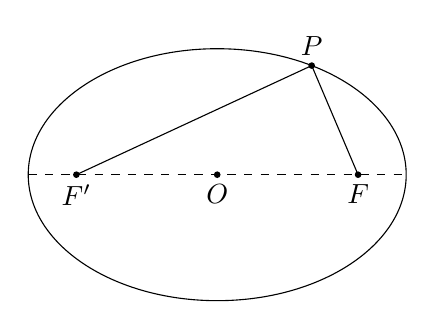
\begin{tikzpicture}[scale=0.8]
                \coordinate (O) at (0,0);
                \coordinate (A) at (3,0);
                \coordinate (Aneg) at (-3,0);
                \coordinate (B) at (0,2);
                \coordinate (Bneg) at (0,-2);
                \coordinate (F) at (2.236,0);
                \coordinate (Fneg) at (-2.236,0);
                \coordinate (P) at (1.5,1.732);

                \draw (O) ellipse (3 and 2);
                \draw[dashed] (Aneg) -- (A);
                % \draw[dashed] (Bneg) -- (B);
                \draw (P) -- (F);
                \draw (P) -- (Fneg);

                \fill (O) circle (1.5pt) node[below]{$O$};
                \fill (F) circle (1.5pt) node[below]{$F$};
                \fill (Fneg) circle (1.5pt) node[below]{$F'$};
                \fill (P) circle (1.5pt) node[above]{$P$};
            \end{tikzpicture}
        \end{center}
        \qscore{6}
    \end{questionparts}
\end{question}

\begin{solution}
    \solutionlayout
    \begin{enumerate}[label=(\alph*),leftmargin=2.4em,itemsep=1em,topsep=0.5em,parsep=0.25em]
        \item
        由椭圆的长轴、短轴长求出半长轴 $a$ 与半短轴 $b$。
        \begin{align*}
            a &= \frac{1.5}{2} = 0.75 \text{ m} \\
            b &= \frac{1}{2} = 0.5 \text{ m}
        \end{align*}
        \hfill (2分)
        \begin{enumerate}[label=(\roman*),leftmargin=2.2em,itemsep=0.7em,topsep=0.35em]
            \item 横截面积为
            \begin{align*}
                S &= \pi ab \\
                &= \pi \times 0.75 \times 0.5 \\
                &= 0.375\pi \\
                &\approx 1.178 \text{ m}^2
            \end{align*}
            \hfill (3分)

            \item 油槽的容量为
            \begin{align*}
                V &= S \times 4 \\
                &= 0.375\pi \times 4 \\
                &= 1.5\pi \text{ m}^3 \\
                &\approx 4.712 \text{ m}^3
            \end{align*}
            \hfill (3分)
            \[
                V \approx 4.712 \times 1000 = 4712 \text{ l}
            \]
            \hfill (2分)
        \end{enumerate}

        \item 求证 $|PF|+|PF'|$ 为定值，并求出该定值。 \\
        设 $P(x,y)$，将 $|PF|$、$|PF'|$ 用坐标表示，并利用椭圆方程消去 $y^2$。 \\
        设 $a=3$，$b=2$，$c^2=a^2-b^2$，则 $F(c,0)$，$F'(-c,0)$。
        \begin{align*}
            c^2 &= 9-4 = 5
        \end{align*}
        \hfill (2分)
        \begin{align*}
            |PF|^2 &= (x-c)^2+y^2 \\
            &= x^2-2cx+c^2+b^2\left(1-\frac{x^2}{a^2}\right) \\
            &= \left(1-\frac{b^2}{a^2}\right)x^2 -2cx+c^2+b^2 \\
            &= \frac{c^2}{a^2}x^2-2cx+a^2 \\
            &= \left(\frac{c}{a}x-a\right)^2
        \end{align*}
        \hfill (3分)
        由 $|x|\le a$ 且 $\dfrac{c}{a}<1$，得 $\dfrac{c}{a}x-a\le 0$，故
        \[
            |PF| = a-\frac{c}{a}x
        \]
        同理可得
        \[
            |PF'| = a+\frac{c}{a}x
        \]
        \hfill (2分)
        \begin{align*}
            |PF|+|PF'| &= \left(a-\frac{c}{a}x\right)+\left(a+\frac{c}{a}x\right) \\
            &= 2a \\
            &= 6
        \end{align*}
        与 $x$ 无关，故 $|PF|+|PF'|$ 为定值 $6$。
        \hfill (1分)
    \end{enumerate}
\end{solution}
%endregion

%region 范围：解析几何（双曲线）| 考点：双曲线标准式化简、几何性质、渐近线族方程 | 难度：中等偏难
\begin{question}[points = 10]
    \begin{questionparts}
        \item 已知一双曲线的方程式为 $16x^2-9y^2+96x-36y-36=0$，求它的中心、对称轴、实轴与虚轴的长、离心率、顶点、焦点、准线及渐近线，并绘其图像。 \qscore{8}

        \item 已知一直角双曲线经过点 $\left(4,\ 1+\sqrt{3}\right)$，且它的渐近线为 $x-y-1=0$ 及 $x+y-3=0$，求其方程式。 \qscore{4}
    \end{questionparts}
\end{question}

\begin{solution}
    \solutionlayout
    \begin{enumerate}[label=(\alph*),leftmargin=2.4em,itemsep=1em,topsep=0.5em,parsep=0.25em]
        \item 求双曲线 $16x^2-9y^2+96x-36y-36=0$ 的中心、对称轴、实轴与虚轴的长、离心率、顶点、焦点、准线及渐近线，并绘其图像。 \\
        先将方程配方，化为标准式，再逐一读出各几何量。
        \begin{align*}
            16x^2+96x-9y^2-36y-36 &= 0 \\
            16(x^2+6x)-9(y^2+4y) &= 36 \\
            16\left[(x+3)^2-9\right]-9\left[(y+2)^2-4\right] &= 36 \\
            16(x+3)^2-9(y+2)^2 &= 36+144-36 \\
            16(x+3)^2-9(y+2)^2 &= 144
        \end{align*}
        两边除以 $144$：
        \[
            \frac{(x+3)^2}{9}-\frac{(y+2)^2}{16}=1
        \]
        \hfill (2分)
        由标准式得 $a^2=9,\ b^2=16$，故 $a=3,\ b=4$，中心为 $(-3,-2)$；实轴为水平方向，对称轴为 $y=-2$（实轴所在直线）及 $x=-3$（虚轴所在直线）。
        \hfill (1分)
        \begin{align*}
            c^2 &= a^2+b^2 = 9+16=25 \implies c=5
        \end{align*}
        实轴长 $=2a=6$，虚轴长 $=2b=8$，离心率 $e=\dfrac{c}{a}=\dfrac{5}{3}$。
        \hfill (1分)
        顶点为 $(-3\pm a,-2)=(0,-2)$ 及 $(-6,-2)$；焦点为 $(-3\pm c,-2)=(2,-2)$ 及 $(-8,-2)$。
        \hfill (1分)
        准线为 $x=-3\pm\dfrac{a^2}{c}=-3\pm\dfrac{9}{5}$，即 $x=-\dfrac{6}{5}$ 及 $x=-\dfrac{24}{5}$。
        \hfill (1分)
        渐近线为 $\dfrac{x+3}{3}=\pm\dfrac{y+2}{4}$，即
        \[
            4x-3y+6=0 \quad \text{及} \quad 4x+3y+18=0
        \]
        \hfill (1分)

        图像如下：
        \begin{center}
            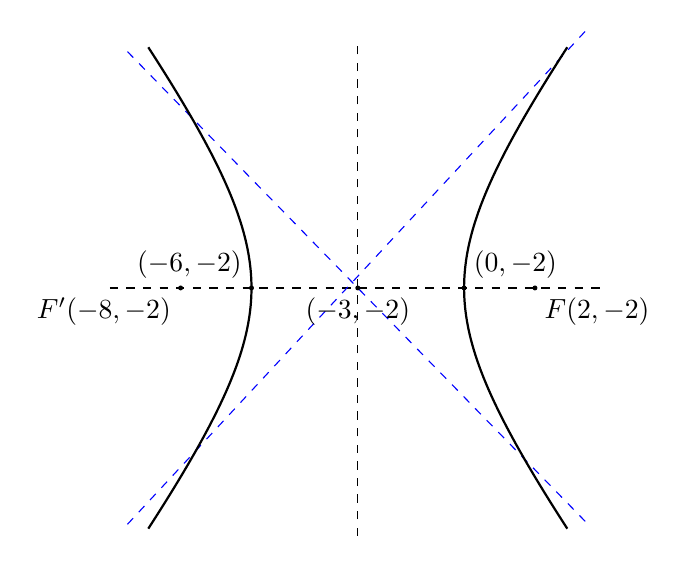
\begin{tikzpicture}[scale=0.45]
                \coordinate (C) at (-3,-2);
                \coordinate (V1) at (0,-2);
                \coordinate (V2) at (-6,-2);
                \coordinate (F1) at (2,-2);
                \coordinate (F2) at (-8,-2);

                \draw[dashed] (-10,-2) -- (4,-2);
                \draw[dashed] (-3,-9) -- (-3,5);

                \draw[dashed,blue] (-9.5,-8.67) -- (3.5,5.33);
                \draw[dashed,blue] (-9.5,4.67) -- (3.5,-8.67);

                \draw[domain=-1.3:1.3,smooth,samples=60,variable=\t,thick]
                    plot ({-3+3*cosh(\t)},{-2+4*sinh(\t)});
                \draw[domain=-1.3:1.3,smooth,samples=60,variable=\t,thick]
                    plot ({-3-3*cosh(\t)},{-2+4*sinh(\t)});

                \fill (C) circle (2pt) node[below]{$(-3,-2)$};
                \fill (V1) circle (2pt) node[above right]{$(0,-2)$};
                \fill (V2) circle (2pt) node[above left]{$(-6,-2)$};
                \fill (F1) circle (2pt) node[below right]{$F(2,-2)$};
                \fill (F2) circle (2pt) node[below left]{$F'(-8,-2)$};
            \end{tikzpicture}
        \end{center}

        \item 求经过点 $\left(4,1+\sqrt{3}\right)$、渐近线为 $x-y-1=0$ 及 $x+y-3=0$ 的直角双曲线方程式。 \\
        由于双曲线的两条渐近线为 $x-y-1=0$ 及 $x+y-3=0$，其方程式可设为 $(x-y-1)(x+y-3)=k$，代入已知点求出 $k$。
        \begin{align*}
            x-y-1 &= 4-(1+\sqrt3)-1 = 2-\sqrt3 \\
            x+y-3 &= 4+(1+\sqrt3)-3 = 2+\sqrt3
        \end{align*}
        \begin{align*}
            k &= (2-\sqrt3)(2+\sqrt3) \\
            &= 4-3 \\
            &= 1
        \end{align*}
        \hfill (2分)
        故所求方程式为
        \[
            (x-y-1)(x+y-3)=1
        \]
        展开化简得
        \[
            x^2-y^2-4x+2y+2=0
        \]
        \hfill (1分)
    \end{enumerate}
\end{solution}
%endregion

%region 范围：复数（棣美弗定理）| 考点：棣美弗定理展开三角恒等式、复数乘法与辐角的应用 | 难度：中等偏难
\begin{question}[points = 12]
    \begin{questionparts}
        \item 利用棣美弗定理证明：$\cos 6\theta = 32\cos^6\theta - 48\cos^4\theta + 18\cos^2\theta - 1$
        \qscore{6}

        \item
        \begin{enumerate}[label=(\roman*),leftmargin=2em,itemsep=0.5em]
            \item 求 $(1+i)(1+2i)(1+3i)$ 的值。\qscore{3}
            \item 利用 (i) 的结果，证明
            $\tan^{-1}1+\tan^{-1}2+\tan^{-1}3=\pi$。\qscore{3}
        \end{enumerate}
    \end{questionparts}
\end{question}

\begin{solution}
    \solutionlayout
    \begin{enumerate}[label=(\alph*),leftmargin=2.4em,itemsep=1em,topsep=0.5em,parsep=0.25em]
        \item 利用棣美弗定理证明 $\cos6\theta=32\cos^6\theta-48\cos^4\theta+18\cos^2\theta-1$。 \\
        由棣美弗定理，$(\cos\theta+i\sin\theta)^6=\cos6\theta+i\sin6\theta$，用二项式定理展开左边并取实部。
        \begin{align*}
            (\cos\theta+i\sin\theta)^6
            &= \cos^6\theta + \binom{6}{1}\cos^5\theta(i\sin\theta) + \binom{6}{2}\cos^4\theta(i\sin\theta)^2 \\
            &\quad + \binom{6}{3}\cos^3\theta(i\sin\theta)^3 + \binom{6}{4}\cos^2\theta(i\sin\theta)^4 \\
            &\quad + \binom{6}{5}\cos\theta(i\sin\theta)^5 + (i\sin\theta)^6
        \end{align*}
        \hfill (1分)
        取实部（即 $(i\sin\theta)^k$ 中 $k$ 为偶数的各项，利用 $i^2=-1,\ i^4=1,\ i^6=-1$）：
        \begin{align*}
            \cos6\theta &= \cos^6\theta - 15\cos^4\theta\sin^2\theta + 15\cos^2\theta\sin^4\theta - \sin^6\theta
        \end{align*}
        \hfill (2分)
        设 $c=\cos\theta$，代入 $\sin^2\theta=1-c^2$：
        \begin{align*}
            \cos6\theta &= c^6 - 15c^4(1-c^2) + 15c^2(1-c^2)^2 - (1-c^2)^3
        \end{align*}
        \hfill (1分)
        展开每一项：
        \begin{align*}
            c^6 &= c^6 \\
            -15c^4(1-c^2) &= -15c^4+15c^6 \\
            15c^2(1-c^2)^2 &= 15c^2-30c^4+15c^6 \\
            -(1-c^2)^3 &= -1+3c^2-3c^4+c^6
        \end{align*}
        \hfill (1分)
        将各项按次数合并：
        \begin{align*}
            \cos6\theta &= (1+15+15+1)c^6 + (-15-30-3)c^4 + (15+3)c^2 - 1 \\
            &= 32c^6-48c^4+18c^2-1
        \end{align*}
        故 $\cos6\theta=32\cos^6\theta-48\cos^4\theta+18\cos^2\theta-1$，得证。
        \hfill (1分)

        \item
        \begin{enumerate}[label=(\roman*),leftmargin=2.2em,itemsep=0.7em,topsep=0.35em]
            \item 计算复数乘积：
            \begin{align*}
                (1+i)(1+2i) &= -1+3i, \\
                (1+i)(1+2i)(1+3i)
                &=(-1+3i)(1+3i) \\
                &=-1-9 \\
                &=-10.
            \end{align*}
            故 $(1+i)(1+2i)(1+3i)=-10$。
            \hfill (3分)

            \item 由于 $1+i$、$1+2i$、$1+3i$ 均在第一象限，故
            \begin{align*}
                \arg(1+i)&=\tan^{-1}1, \\
                \arg(1+2i)&=\tan^{-1}2, \\
                \arg(1+3i)&=\tan^{-1}3.
            \end{align*}
            根据辐角的加法性质，
            \begin{align*}
                &\tan^{-1}1+\tan^{-1}2+\tan^{-1}3 \\
                &\quad=\arg\big[(1+i)(1+2i)(1+3i)\big] \\
                &\quad=\arg(-10)=\pi.
            \end{align*}
            因此
            \[
                \tan^{-1}1+\tan^{-1}2+\tan^{-1}3=\pi.
            \]
            \hfill (3分)
        \end{enumerate}
    \end{enumerate}
\end{solution}
%endregion

%region 范围：复数方程、复数的 n 次方根 | 考点：实系数多项式的共轭虚根、棣美弗定理求 n 次方根 | 难度：中等偏难
\begin{question}[points = 12]
    \begin{questionparts}
        \item 已知 $1+2i$ 是方程式 $x^4-x^3-3x^2+17x-30=0$ 的根，解这个方程式。 \qscore{6}

        \item 解方程 $(x-i)^5=i$。 \qscore{6}
    \end{questionparts}
\end{question}

\begin{solution}
    \solutionlayout
    \begin{enumerate}[label=(\alph*),leftmargin=2.4em,itemsep=1em,topsep=0.5em,parsep=0.25em]
        \item 已知 $1+2i$ 是方程式 $x^4-x^3-3x^2+17x-30=0$ 的根，解这个方程式。 \\
        由于该方程系数皆为实数，虚根必成共轭对出现，故 $1-2i$ 也是方程的根，可先求出对应的二次因式。
        \begin{align*}
            \big[x-(1+2i)\big]\big[x-(1-2i)\big] &= (x-1)^2-(2i)^2 \\
            &= x^2-2x+1+4 \\
            &= x^2-2x+5
        \end{align*}
        \hfill (2分)
        以 $x^2-2x+5$ 除原方程左边的四次式，求出另一二次因式：
        \[
            x^4-x^3-3x^2+17x-30 = (x^2-2x+5)(x^2+x-6)
        \]
        \hfill (2分)
        将 $x^2+x-6$ 因式分解：
        \[
            x^2+x-6=(x+3)(x-2)
        \]
        故方程的四个根为
        \[
            x=1+2i,\quad x=1-2i,\quad x=-3,\quad x=2
        \]
        \hfill (2分)

        \item 解方程 $(x-i)^5=i$。 \\
        设 $y=x-i$，则 $y^5=i$，先将 $i$ 化为极坐标（三角）形式。
        \[
            i=\cos90^\circ+i\sin90^\circ
        \]
        \hfill (1分)
        由棣美弗定理，$y^5=i$ 的一般辐角为 $90^\circ+360^\circ k$。令
        \[
            \theta_k=\frac{90^\circ+360^\circ k}{5}
            =18^\circ+72^\circ k,
            \qquad k=0,1,2,3,4,
        \]
        则五个五次方根为
        \[
            y_k=\cos\theta_k+i\sin\theta_k,
            \qquad k=0,1,2,3,4.
        \]
        \hfill (2分)
        代入 $k=0,1,2,3,4$，得五个 $y$ 值，对应辐角为 $18^\circ,\ 90^\circ,\ 162^\circ,\ 234^\circ,\ 306^\circ$：
        \begin{align*}
            y_0 &= \cos18^\circ+i\sin18^\circ \\
            y_1 &= \cos90^\circ+i\sin90^\circ = i \\
            y_2 &= \cos162^\circ+i\sin162^\circ \\
            y_3 &= \cos234^\circ+i\sin234^\circ \\
            y_4 &= \cos306^\circ+i\sin306^\circ
        \end{align*}
        \hfill (2分)
        由 $x=y+i$，得方程的五个根：
        \begin{align*}
            x_0 &= \cos18^\circ+i(\sin18^\circ+1) \\
            x_1 &= 2i \\
            x_2 &= \cos162^\circ+i(\sin162^\circ+1) \\
            x_3 &= \cos234^\circ+i(\sin234^\circ+1) \\
            x_4 &= \cos306^\circ+i(\sin306^\circ+1)
        \end{align*}
        \hfill (1分)
    \end{enumerate}
\end{solution}
%endregion

%region 范围：向量、空间坐标 | 考点：向量数量积、向量垂直的条件、空间两点距离公式 | 难度：中等
\begin{question}[points = 12]
    \begin{questionparts}
        \item 已知 $|\underline{a}|=4$，$|\underline{b}|=2$，向量 $2\underline{a}+\underline{b}$ 与向量 $\underline{a}-3\underline{b}$ 互相垂直，求向量 $\underline{a}$ 与向量 $\underline{b}$ 的夹角。 \qscore{7}

        \item 若点 $P(3,7,h+2)$ 与点 $Q(-h,1,7)$ 之间的距离为 $10$，求 $h$ 的值。 \qscore{5}
    \end{questionparts}
\end{question}

\begin{solution}
    \solutionlayout
    \begin{enumerate}[label=(\alph*),leftmargin=2.4em,itemsep=1em,topsep=0.5em,parsep=0.25em]
        \item 已知 $|\underline{a}|=4,\ |\underline{b}|=2$，$2\underline{a}+\underline{b}$ 与 $\underline{a}-3\underline{b}$ 互相垂直，求 $\underline{a}$ 与 $\underline{b}$ 的夹角。 \\
        两向量垂直，其数量积为零，先展开 $(2\underline{a}+\underline{b})\cdot(\underline{a}-3\underline{b})=0$。
        \begin{align*}
            (2\underline{a}+\underline{b})\cdot(\underline{a}-3\underline{b})
            &= 2(\underline{a}\cdot\underline{a})-6(\underline{a}\cdot\underline{b}) \\
            &\quad +(\underline{a}\cdot\underline{b})-3(\underline{b}\cdot\underline{b}) \\
            &= 2|\underline{a}|^2 - 5(\underline{a}\cdot\underline{b}) - 3|\underline{b}|^2 \\
            &= 0
        \end{align*}
        \hfill (2分)
        代入 $|\underline{a}|=4,\ |\underline{b}|=2$：
        \begin{align*}
            2(4)^2 - 5(\underline{a}\cdot\underline{b}) - 3(2)^2 &= 0 \\
            32 - 5(\underline{a}\cdot\underline{b}) - 12 &= 0 \\
            \underline{a}\cdot\underline{b} &= 4
        \end{align*}
        \hfill (2分)
        设 $\underline{a}$ 与 $\underline{b}$ 的夹角为 $\theta$，由 $\underline{a}\cdot\underline{b}=|\underline{a}||\underline{b}|\cos\theta$：
        \begin{align*}
            \cos\theta &= \frac{\underline{a}\cdot\underline{b}}{|\underline{a}||\underline{b}|} \\
            &= \frac{4}{4\times2} \\
            &= \frac{1}{2}
        \end{align*}
        \[
            \theta = \cos^{-1}\left(\frac{1}{2}\right) = 60^\circ
        \]
        \hfill (2分)

        \item 若点 $P(3,7,h+2)$ 与点 $Q(-h,1,7)$ 之间的距离为 $10$，求 $h$。 \\
        由空间两点距离公式，代入坐标并令其等于 $10$。
        \begin{align*}
            \sqrt{\big(3-(-h)\big)^2+(7-1)^2+\big((h+2)-7\big)^2} &= 10
        \end{align*}
        \hfill (2分)
        两边平方，展开化简：
        \begin{align*}
            (3+h)^2+6^2+(h-5)^2 &= 100 \\
            (h^2+6h+9)+36+(h^2-10h+25) &= 100 \\
            2h^2-4h+70 &= 100 \\
            2h^2-4h-30 &= 0 \\
            h^2-2h-15 &= 0
        \end{align*}
        \hfill (2分)
        因式分解：
        \[
            (h-5)(h+3)=0
        \]
        故
        \[
            h=5 \quad \text{或} \quad h=-3
        \]
        \hfill (2分)
    \end{enumerate}
\end{solution}
%endregion

%region 范围：空间向量 | 考点：向量叉乘求平行四边形面积、线段外分点坐标公式 | 难度：中等
\begin{question}[points = 12]
    \begin{questionparts}
        \item 已知平行四边形 $ABCD$，其中三个顶点为 $A(2,1,0)$，$B(3,3,1)$ 及 $D(1,2,2)$，求其面积。 \qscore{6}

        \item 已知 $P(2,1,-1)$，$Q(10,5,3)$ 两点，求将线段 $PQ$ 外分成 $1:3$ 的点 $R$ 的坐标。 \qscore{6}
    \end{questionparts}
\end{question}

\begin{solution}
    \solutionlayout
    \begin{enumerate}[label=(\alph*),leftmargin=2.4em,itemsep=1em,topsep=0.5em,parsep=0.25em]
        \item 已知平行四边形 $ABCD$ 三个顶点 $A(2,1,0)$，$B(3,3,1)$，$D(1,2,2)$，求其面积。 \\
        在平行四边形 $ABCD$ 中，$AB$ 与 $AD$ 为顶点 $A$ 处的两条邻边，先求出这两个向量。
        \begin{align*}
            \overrightarrow{AB} &= B-A = (1,2,1) \\
            \overrightarrow{AD} &= D-A = (-1,1,2)
        \end{align*}
        \hfill (2分)
        平行四边形的面积等于 $\big|\overrightarrow{AB}\times\overrightarrow{AD}\big|$，先求叉积：
        \begin{align*}
            \overrightarrow{AB}\times\overrightarrow{AD}
            &= \begin{vmatrix} \mathbf{i} & \mathbf{j} & \mathbf{k} \\ 1 & 2 & 1 \\ -1 & 1 & 2 \end{vmatrix} \\
            &= \big(2(2)-1(1)\big)\mathbf{i} - \big(1(2)-1(-1)\big)\mathbf{j} + \big(1(1)-2(-1)\big)\mathbf{k} \\
            &= 3\mathbf{i}-3\mathbf{j}+3\mathbf{k} \\
            &= (3,-3,3)
        \end{align*}
        \hfill (2分)
        求其模长即得面积：
        \begin{align*}
            \text{面积} &= \big|\overrightarrow{AB}\times\overrightarrow{AD}\big| \\
            &= \sqrt{3^2+(-3)^2+3^2} \\
            &= \sqrt{27} \\
            &= 3\sqrt{3} \text{ 平方单位}
        \end{align*}
        \hfill (2分)

        \item 已知 $P(2,1,-1)$，$Q(10,5,3)$，求将线段 $PQ$ 外分成 $1:3$ 的点 $R$ 的坐标。 \\
        设 $R$ 将 $PQ$ 外分成 $m:n=1:3$，则 $R$ 的坐标公式为
        \[
            R=\frac{nP-mQ}{n-m}
        \]
        \hfill (1分)
        代入 $P(2,1,-1)$，$Q(10,5,3)$，$m=1,\ n=3$：
        \begin{align*}
            R &= \frac{3P-Q}{3-1} \\
            &= \frac{3(2,1,-1)-(10,5,3)}{2} \\
            &= \frac{(6,3,-3)-(10,5,3)}{2} \\
            &= \frac{(-4,-2,-6)}{2}
        \end{align*}
        \hfill (3分)
        故
        \[
            R=(-2,-1,-3)
        \]
        \hfill (2分)
    \end{enumerate}
\end{solution}
%endregion





%region 签名栏
\vfill % 与上方内容保持距离

\noindent
\newlength{\sigwidth}
\settowidth{\sigwidth}{（\hspace{4em}师）}

\begin{tabular*}{\textwidth}{@{\extracolsep{\fill}} l l l}
    出题： & 审题： & 审核： \\[4em]
    \rule{\sigwidth}{0.5pt} &
    \rule{\sigwidth}{0.5pt} &
    \rule{\sigwidth}{0.5pt} \\
    （\hspace{0em} \setterteacher ） &
    （\hspace{0em} \reviewteacher ）  &
    （\hspace{0em} \auditteacher ） \\
\end{tabular*}
%endregion

\newpage
\end{document}